\documentclass[../statistical_learning_notes.tex]{subfiles}
\begin{document}
%%%%%%%%%%%%%%%%%%%%%%%%%%%%%%%%%%%%%%%%%%%%%%%%%%%%%%%%%%%%%%%%%%%%%%%%%%%
\chapter{Bayesian Methods}
The Bayes formula will be invaluable throughout the analysis of Bayesian methods in Machine Learning. Suppose we observe $N$ data points jointly represented by $X$ and we know that they come from a distribution with parameters $\theta$, then
\begin{align*}
    P(\theta|X) = \frac{P(X|\theta)P(\theta)}{P(X)}
\end{align*}
where
\begin{itemize}
    \item $P(\theta|X)$ is called the posterior, the probability distribution of $\theta$ having observed the data
    \item $P(X|\theta)$ is called the likelihood, the probability of occurence of the data under a given $\theta$
    \item $P(\theta)$ is called the prior, our prior beliefs about the parameters without seeing the data
    \item $P(X)$ is the probability distribution of the data which is fixed for a given data set
\end{itemize}


\subfile{bayesian_methods/mle}
\subfile{bayesian_methods/map}

%%%%%%%%%%%%%%%%%%%%%%%%%%%%%%%%%%%%%%%%%%%%%%%%%%%%%%%%%%%%%%%%%%%%%%%%%%%
\subsection{Conjugate Distributions}
Conjugate distributions are really helpful in calculating the posterior, especially in case of complicated distributions. In the context of MAP estimate, the prior is said to be the \textbf{conjugate prior} of the likelihood if the \textbf{posterior} obtained by multiplying the likelihood \textbf{and the prior belong to the same family of distributions}. An example
\begin{gather*}
    p(X|\theta) = \mathcal{N}(\alpha_{1}, \beta_{1}^{2}), \quad p(\theta) = \mathcal{N}(\alpha_{2}, \beta_{2}^{2})\\
    \text{Then,} \quad p(\theta|X) \propto p(X|\theta)p(\theta) = \mathcal{N}(\alpha_{3}, \beta_{3}^{2})
\end{gather*}
which stems from the simple fact that multiplication of two normals will sum up the exponential terms, resulting in a constant times a new normal distribution. We ignore the constant since we only need the functional form for optimization.\newline
\textbf{Normal distribution is conjugate to the normal distribution}.


%%%%%%%%%%%%%%%%%%%%%%%%%%%%%%%%%%%%%%%
\subfile{bayesian_methods/em}
\subfile{bayesian_methods/variational_inference}
%%%%%%%%%%%%%%%%%%%%%%%%%%%%%%%%%%%%%%%

\section*{Comparison of Different Inference Methods}
\begin{figure}[h]
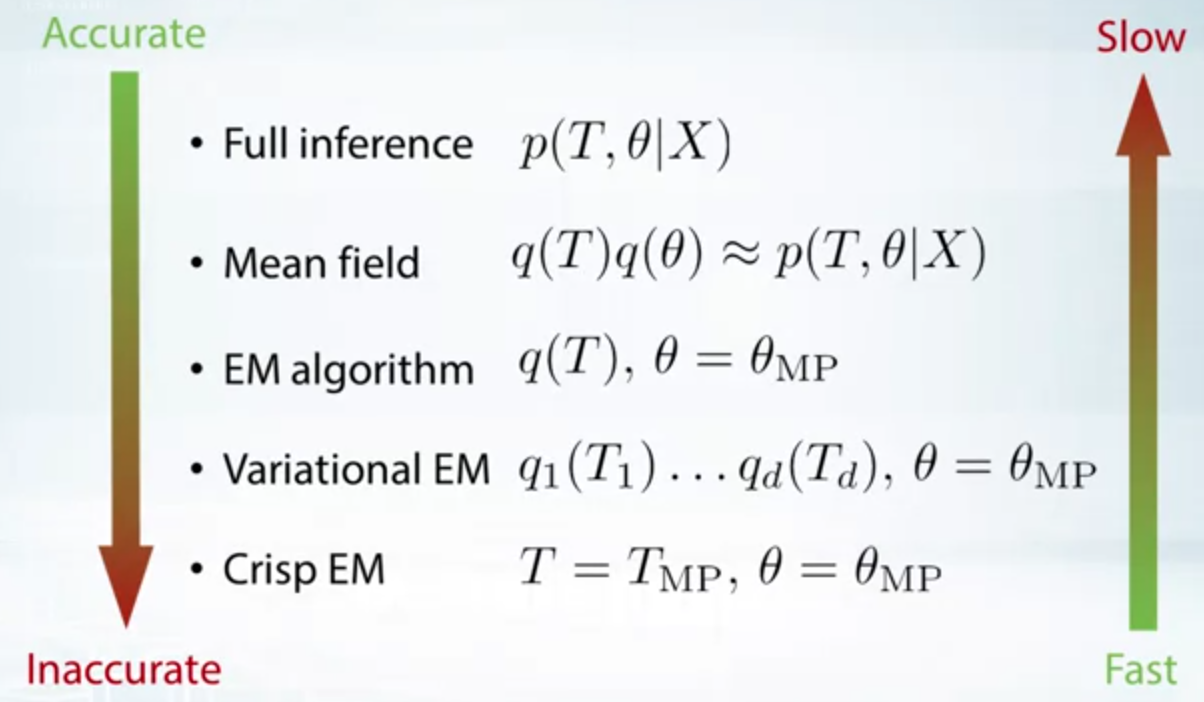
\includegraphics[scale=0.3]{em_2}
\centering
\caption{Comparison of different inference methods in terms of accuracy and inference speed}
\label{fig:em_2} %\ref{fig:em_2}
\end{figure}

%%%%%%%%%%%%%%%%%%%%%%%%%%%%%%%%%%%%%%%
\subfile{bayesian_methods/lda}
\subfile{bayesian_methods/probabilistic_sampling}
\end{document}